%!TeX root=../tese.tex
%("dica" para o editor de texto: este arquivo é parte de um documento maior)
% para saber mais: https://tex.stackexchange.com/q/78101

%% ------------------------------------------------------------------------- %%

% "\chapter" cria um capítulo com número e o coloca no sumário; "\chapter*"
% cria um capítulo sem número e não o coloca no sumário. Alguns autores
% preferem que a introdução não seja numerada, mas ainda assim apareça
% no sumário. Para isso, você pode usar "\chapter**{Introdução}". Esse
% comando não é padrão do LaTeX; ele foi definido neste modelo.
\chapter{Introdução}
\label{cap:introducao}

Sistemas de detecção de intrusão (IDS – Intrusion Detection System) utilizam informações de diversas camadas da arquitetura Internet presentes em pacotes de rede para alertar sobre potenciais ataques ocorrendo em uma rede de computadores. Embora haja ressalvas relacionadas à privacidade quando da utilização de informações das camadas superiores ~\citep{daniel-privacidade}, o protocolo DNS (\textit{Domain Name System}) tradicionalmente é transportado sem criptografia pelas redes, podendo auxiliar na detecção de ataques. Por exemplo, a detecção imediata de dispositivos de uma rede acessando nomes de domínio criados exclusivamente para hospedar códigos maliciosos (\textit{malware}) ou para hospedar cópias de sites oficiais com o objetivo de obter, de forma ilegal, credenciais de acesso aos sites originais (\textit{phishing}) pode ser usada como gatilho para a criação de uma regra em um \textit{firewall} ou em um servidor DNS para impedir que o tráfego suspeito seja realizado. Entretanto, nomes de domínio criados com intenção maliciosa ocorrem a todo momento e detectar essas criações de forma antecipada é algo difícil de ser realizado sem algum mecanismo automatizado. Mesmo que essa detecção ocorra, o processo burocrático para “derrubar” os domínios toma tempo, justificando mecanismos de mitigação que atuem diretamente nos dispositivos de interconexão.

Para exemplificar tal problema, a Superintendência de Tecnologia da Informação da USP detectou a criação de um clone do Portal de Serviços da USP no nome de domínio \texttt{uspdigital.com.br}  (Figura~\ref{fig:usp-clone}) e informou a comunidade da Universidade a respeito no dia 3 de Junho de 2025. O serviço de registros responsável pelo domínio e outras autoridades foram informadas sobre o ocorrido, mas mesmo 12 dias após, o domínio continua no ar.

\begin{figure}[htb]
\centering
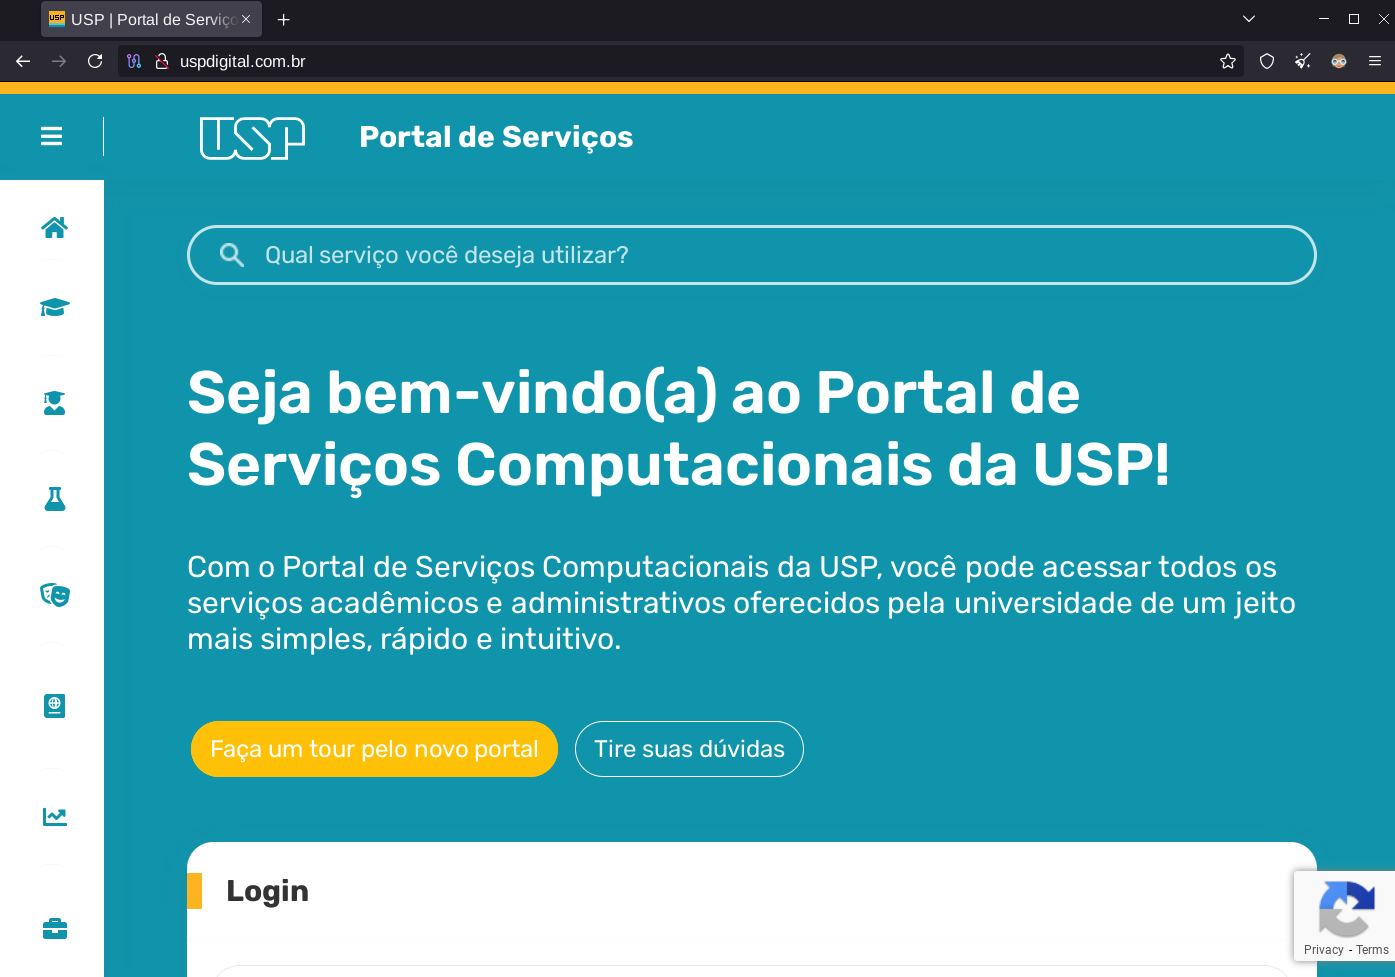
\includegraphics[width=.7\textwidth]{figuras/site-falso-usp.png}
\caption{Captura de tela da página hospedada em \texttt{uspdigital.com.br}}\label{fig:usp-clone}
\end{figure}

Um procedimento para mitigar esse problema consiste (1) na captura do tráfego DNS; (2) no processamento do mesmo por meio de algum mecanismo de aprendizado de máquina que identifique nomes de domínio maliciosos; e (3) na criação de regras em servidores DNS ou \textit{firewalls} para impedir que o tráfego para esses domínios tenha sucesso.

Esta monografia descreve a execução de todas as atividades planejadas para o trabalho de conclusão do curso de bacharelado em Ciência da Computação intitulado \emph{Um Sistema Baseado em Redes Neurais para Detecção de Intrusão em Tráfego DNS}.

Este trabalho fez parte do  CPE SMARTNESS (FAPESP 21/00199-8) e foi, também, suportado pelo projeto FAPESP 25/22251-2, desenvolvido no Departamento de Ciência da Computação do IME-USP.

\section**{Objetivos e Contribuições}

O projeto teve como objetivo principal o desenvolvimento de um mecanismo de detecção de domínios maliciosos baseado em redes neurais, utilizando como entrada o tráfego do protocolo DNS, com foco na especialização do modelo para o contexto brasileiro (nomes de domínios terminados em .br), algo útil, por exemplo, para detectar antecipadamente casos como o que ocorreu com o Portal de Serviços da USP. Como objetivos secundários também foram realizados: aplicação de \textit{feature engineering} por meio do estudo de explicabilidade e comparação do desempenho do mecanismo com outros modelos para classificação de tráfego.

Resultados obtidos com a utilização do mecanismo na detecção de domínios maliciosos presentes no dataset BCCC-CIC-Bell-DNS-2024 \citep{dataset-site} \citep{SHAFI2024109436}, um dataset criado para modelar o perfil comportamental de diferentes atividades de DNS, mostraram que a etapa de explicabilidade foi fundamental para identificar \textit{features} irrelevantes, levando o modelo a detectar tráfego benigno com F1-Score médio de 0,95 e tráfego malicioso com F1-Score médio de 0,82.

Entre outros resultados diretos do trabalho, destacam-se:
\begin{itemize}
    \item a publicação do artigo científico intitulado \emph{Detecção de Intrusões em Tráfego DNS utilizando Redes Neurais e Explicabilidade} \citep{hirata2026dns} nos Anais Estendidos do XLIV Simpósio Brasileiro de Redes de Computadores e Sistemas Distribuídos (SBRC 2026);
    \item a disponibilização de todo o código desenvolvido como software livre no repositório (\url{https://github.com/giovannahirata/IDS-DNS}).
\end{itemize}

\section**{Eixo de Extensão}

Ao priorizar a análise e identificação proativa de domínios maliciosos no tráfego DNS, este sistema proposto beneficia os usuários finais da Internet ao bloquear conexões antes da consolidação do ataque, prevenindo infecções por códigos maliciosos \textit{malware} e o roubo de credenciais em fraudes de \textit{phishing}. No entanto, para avaliar o resultado prático e a usabilidade do IDS, delimitou-se o grupo amostral a fim de construir um diálogo mais próximo e medir o real impacto de utilizar o sistema proposto para evitar acidentes cibernéticos.

Por isso, a questão social abordada focou em indivíduos com menor grau de letramento digital frente às questões de segurança nas redes e internet, priorizando usuários sem formação na área de Tecnologia da Informação e, preferencialmente, de faixas etárias mais elevadas. Esse grupo atuou de forma participativa ao longo do ciclo de desenvolvimento, por meio do preenchimento de questionários avaliativos sobre a percepção de legitimidade de URLs reais (documentados no Apêndice~\ref{ap:formulario}).

O retorno obtido orientou os ajustes na explicabilidade e engenharia de atributos do modelo, assegurando que nomes de domínio com aparência legítima para o público leigo fossem devidamente identificados pela arquitetura neural. Dessa forma, além da validação técnica tradicional por métricas de classificação (como acurácia, precisão, \textit{recall} e \textit{F1-Score}), o projeto incorpora a validação humana como referência de eficácia, buscando reduzir o prejuízo financeiro e psicológico decorrente de golpes digitais no cenário nacional.

\section**{Organização da Monografia}

O restante deste documento está estruturado de acordo com as etapas das atividades previstas no cronograma do plano de trabalho:
\begin{itemize}
    \item O \textbf{Capítulo~\ref{cap:conceitos-basicos}} fornece a fundamentação teórica sobre o protocolo DNS e arquiteturas de redes neurais;
    \item O \textbf{Capítulo~\ref{cap:revisao-literatura}} apresenta o levantamento bibliográfico atualizado; 
    \item O \textbf{Capítulo~\ref{cap:datasets}} descreve os conjuntos de dados investigados e os procedimentos de extração e tratamento dos fluxos de tráfego DNS;
    \item O \textbf{Capítulo~\ref{cap:modelo}} detalha a arquitetura do modelo neural proposto, o mecanismo de explicabilidade e a metodologia do eixo de extensão;
    \item O \textbf{Capítulo~\ref{cap:analise-resultados}} expõe os experimentos, os resultados do modelo obtidos com os dados de treinamento e de validação;
    \item O \textbf{Capítulo~\ref{cap:resultados-extensao}} compara os resultados obtidos do modelo com a análise dos formulários aplicados ao público externo;
    \item O \textbf{Capítulo~\ref{cap:conclusao}} sintetiza as conclusões alcançadas e propõe trabalhos futuros;
    \item O \textbf{Apêndice~\ref{ap:formulario}} disponibiliza a íntegra do formulário e a lista dos 200 domínios submetidos à avaliação do público leigo no eixo de extensão.
\end{itemize}